\section{Framework overview}
\label{sec:framework}
This section describes the work which was done at software level which is definitely not a part that can be neglected when working in group on such a complex machine learning project (a lot of heavy computation power required, long training times for limited chances for improvements).  We describe the constraints we had to face and the solutions we found to overcome them. We trained nearly a hundred experiments which requires good organization and a way to track and monitor everything.
We came out with a convenient solution which allows respecting all the project constraints and allows to focus on the machine learning part of the project which will be presented in a latter section.


\subsection*{Constraints statement}
\label{sec:Constraints}
As this work was to  be done in group, we have to develop a framework so everyone could work and share their code independently.
\begin{itemize}
    \item Heterogeneous environments: several operating systems (linux, windows, macOS), various platforms (local laptop training, Kaggle Kernels notebook, remote machines at Ecole Polytechnique). On every platform, data has to be acessible and experiments results have to be stored in a way they can be retrieved. We used the Kaggle dataset feature to  host the raw dataset aswell as the preprocessed data.
    \item Privacy: as not sharing code was among the rules of the challenge, our source code remained private on GitHub (\textit{which made cloning operations even trickier when using Kaggle kernels}).
    \item Reproducibility: all our experiments are reproducible (source code tracking under git, local and cloud storage of experiments results using ~\href{https://wandb.ai/molecule-nlp-altegrad-23/molecule-nlp}{Weights and biases}).
    \item Cost: project total budget limit to 50euros. \textit{Google Collab would not have met this requirements considering the amount of experiments we did and the long training times}.
\end{itemize}


We wrote a framework which takes and solves all these constraints at once and allows to focus on training models.

\subsection*{Definition of an experiment}
An experiment is defined by a unique identifier and the instanciation of a model (tokenization method, architecture of the LLM and GNN), the configuration of an  optimizer and training hyper parameters. At inference time, we're using this unique identifier so we can safely instantiate a network and reload the weights (\textit{trained model are by construction compatible with inference. This avoids the risk of having a `.pth` weight file without knowning which architecture to use to reload it.}).
Launching the training of an experiment goes seamlessly with the following command line, below is the example for experiment 620:
\begin{verbatim}
    python train.py -e 620
\end{verbatim}

The same exact training can be ran directly on Kaggle using their API.
\begin{verbatim}
    python remote_training.py -e 620 -p -nb mol-nlp
\end{verbatim}
Finally, the evaluation mechanism generates the submission csv file and the right Kaggle API command line which can be used to submit to the hosted challenge (with a message which allows to know exactly which experiment was submitted in which conditions).

\begin{verbatim}
python evaluation.py -e 620
\end{verbatim}

\begin{figure}
    \centering
    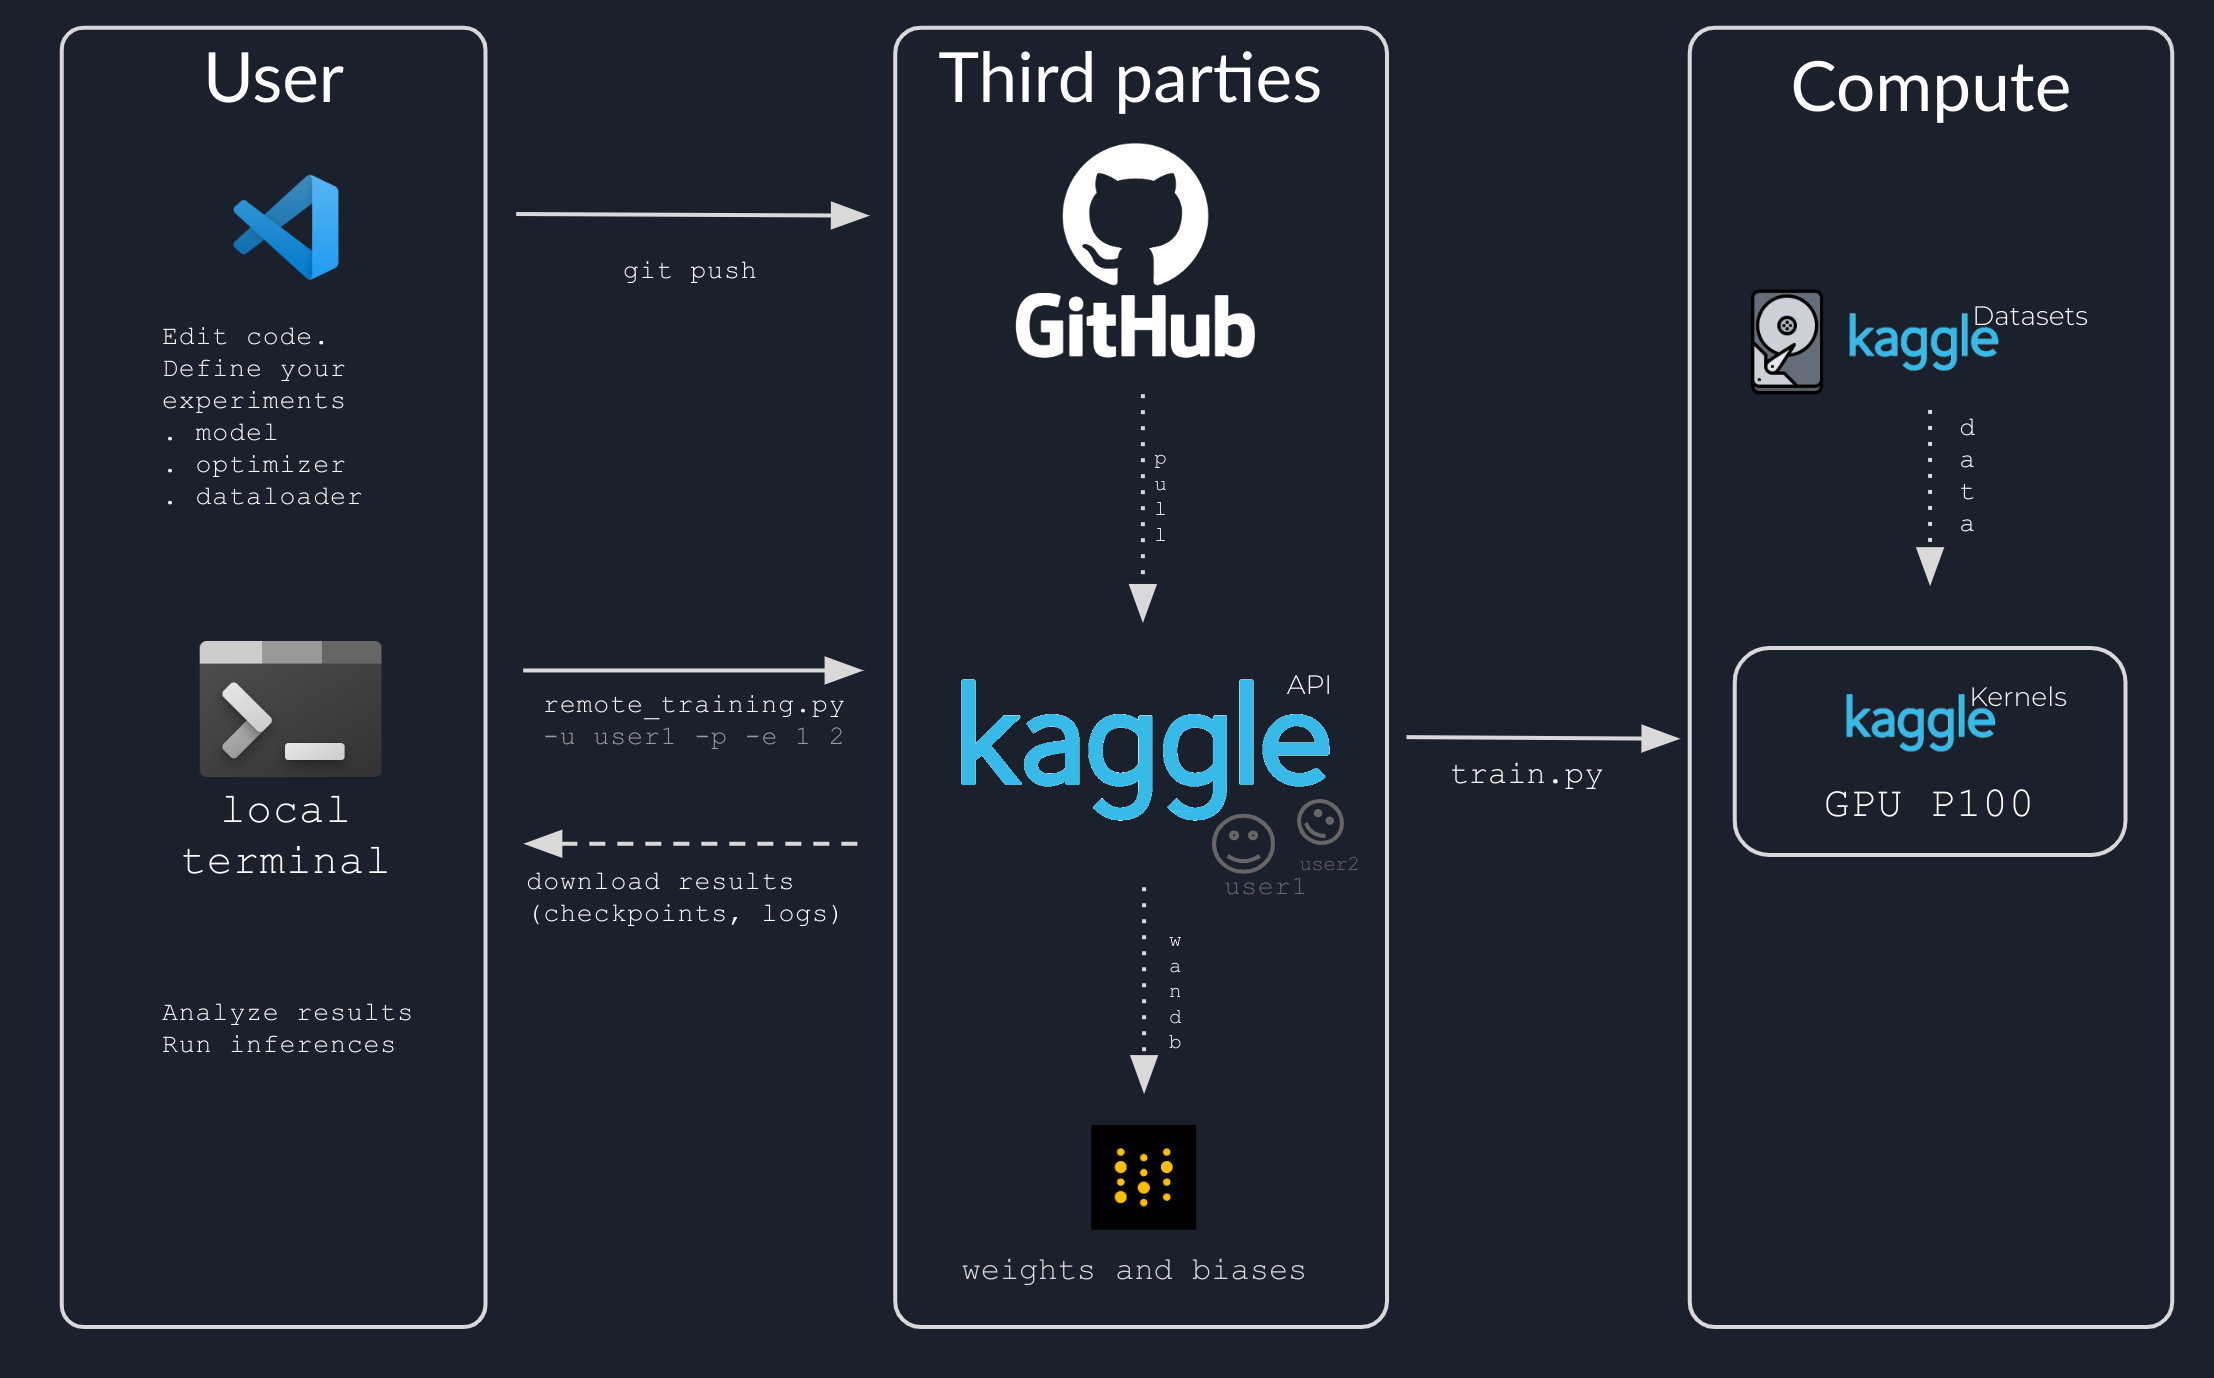
\includegraphics[width=0.5\textwidth]{figures/training_framework.png}
    \caption{Remote training framework allows accessing free GPU resources on Kaggle Kernels. Local code is synchronized through our \textbf{private Github repository} (until the 4th of February) so the remote notebook can be run with the same code. The \textbf{Kaggle dataset} feature is used to store the raw dataset and the preprocessed data (for each tokenizer, we have stored the preprocessed dataset which saves nearly 10 minutes of computation time at the begining of each experiment). The \textbf{Weights and biases} platform is used to track the experiments results and monitor the training. Once finished, trained models can be retrieved by pulling the results.
    Note that the small piece of code to help access \href{https://github.com/balthazarneveu/mva\_pepites}{Kaggle notebooks freely from the terminal} was made available publicly (totally independantly from this challenge) to be later used on other projects.}
    \label{fig:framework}
\end{figure}

\subsection*{Training conditions}
\label{sec:training conditions}

\begin{table*}[ht]
    \centering
    \begin{tabular}{lcccc}
    \hline
    \textbf{Feature} & \textbf{Nvidia T500} & \textbf{Nvidia RTX 2060} & \textbf{Nvidia K100} & \textbf{Nvidia A4000} \\ \hline
    OS & Linux & Linux WSL & Linux in Docker & Linux \\  
    Location            & local laptop           & local laptop  & Kaggle  & Ecole Polytechnique  \\
    Access & direct & direct & Kaggle Kernels & SSH \\
    Dataset access & local SSD & local SSD & Kaggle dataset & remote download + SSD drives\\ 
    Memory           & 4 GB                        & 6 GB                           & 16 GB                          & 24 GB                          \\
    Student cost & - & Electricity $\approx$ +20 euros/month & Free & Free \\
    Availability & $\infty$ & $\infty$ & 30 hours/week 12hours/experiment & $\approx \infty$ weekends and night \\
    \hline
    \end{tabular}
    \caption{Comparison of the training platform and GPUs which were used during training}
    \label{table:gpu_comparison}
\end{table*}


To setup the training loop, we started on a single NVIDIA GeForce RTX T500 local GPU with 4Gb of RAM (\textit{the baseline provided by the challenge organizers did not even run because of memory limitation}). This was enough to make sure we could train, track and monitor progress of all our experiments and build a whole local training framework. We started by freezing the LLM weights to reduce the amount of memory required and get decent batch sizes even on the tiny T500 GPU. Due to low performances, the need to access bigger computation resources quickly came so we had to overcome this difficulty by making our framework agnostic to the training platform and still be able to recover our results and monitor from anywhere. The diversity of training and hardware platforms is shown in \ref*{table:gpu_comparison}. We considered using Google Colab Pro (datasets and models shared through Google drive) but with the consideration that we have long training times, the cost would have been prohibitive. We found a good compromise and did many experiments using Kaggle Kernels through the API which are free and provide GPU acess with 16Gb of RAM during a maximum time of 12 hours per session and up to 30hours per week.



\pagebreak

\section{Our work}
\subsection*{Preliminary study}
\label{sec:preliminary study}

\begin{table*}[h]
    \centering
    \begin{tabular}{|c|c|c|c|c|}
    \hline
    \textbf{Experiment ID} & \textbf{Model Size} & \textbf{LLM} & \textbf{GNN} & \textbf{LRAP} \\ \hline
    101         & 593k                & Frozen Distill-Bert           & Base 3 layer GCN       & 18.7\%      \\ \hline
    106         & 964k                & Frozen Distill-Bert + Adapter & Base 3 layer GCN       & 26.8\%      \\ \hline
    114         & 2.125M              & Frozen Distill-Bert + Adapter & Big 5 layer GCN        & 31.6\%      \\ \hline
    112         & 964k                & Frozen Sci-Bert + Adapter     & Base 3 layer GCN       & 36.7\%      \\ \hline
    113         & 2.125M              & Frozen Sci-Bert + Adapter     & Big 5 layer GCN        & 39.8\%      \\ \hline
    65          & 66.9M               & Trainable Bert                & Base 3 layer GCN       & 63.5\%      \\ \hline
    400         & 110M                & Trainable Sci-Bert            & Base 3 layer GCN       & 66\%        \\ \hline
    \end{tabular}
    \caption{Base Models Specifications and Performances}
    \label{tab:preliminary_study_metrics}
\end{table*}


We start with a few toy experiments to see which architecture factors are most promising (initial hope is that the performances will scale accordingly when we add all extra machine learning tricks).
\textbf{Frozen LLM weights}: We first started with by simple models based on the base GCN (3 graph convolution layers followed by a global pooling layer and 2 layers MLP). Instead of fine tuning all parameters of the LLM, we first started by freezing the LLM parameters. Although simple, this idea intuivitely has many advantages for traing:
\begin{itemize}
    \item We discard the huge memory cost of training a LLM (memory issues not only come from storing the weigths on the GPU but all the optimizers variables during backpropagation). The idea could have been pushed further by pre-computing the text embeddings and storing them on disk. 
    \item Intuivitely, freezing the LLM parameters should make the training more stable as the LLM embeddings acts as a kind of anchor that the GNN shall match.
\end{itemize}
Unfortunately, training achieves low accuracy although the number of parameters to train is lightweight. We added an "adapter" module which is simply a MLP which will adapt by projecting the text representations into a more adapted space which can match with the graph.
\textbf{Influence of the graph neural network size}: We pursued our explorations to see the impact of the GNN size. The \textbf{big GCN} (5 graph convolution layers with 2 residual connection) is more complex and has more parameters to train. We can see that the accuracy is improved by increasing the GCN size. 
\begin{itemize}
    \item Using frozen Distil-BERT: from experiment 106 (base GCN $\text{LRAP}=26.8\%$) to 114 - (big GCN $\text{LRAP}=31.6\%$)
    \item Using frozen SciBERT: from experiment 102 (base GCN $\text{LRAP}=36.7\%$) to 113 - (big GCN $\text{LRAP}=39.8\%$)
\end{itemize}


\textbf{Influence of the pretrained language model}: We also browsed Hugging Face to find models that could be dedicated to scientific-specific language processing. We foud the Sci-Bert\cite{scibert} model and could use it as a drop-in replacement for the Distil-Bert baseline model. Improvements were two-fold when changing the pretrained LLM during this preliminary study: a tokenizer dedicated to a scientific corpus seems by nature a natural choice for scientific words...here atoms and molecule names not being too frequent in common language. The Sci-Bert model may also have reasoning capabilities closer to science and chemistry reactions. This was translated by a improvement in performances. Increasing the GNN size improves accuracy.
\begin{itemize}
    \item Using the Base GCN : from experiment 106 Distil-BERT ($\text{LRAP}=26.8\%$) to experiment 112 - SciBert ($\text{LRAP}=36.7\%$).
    \item Using the Big-GCN: from experiment 114 Distil-BERT ($\text{LRAP}=31.6\%$) to experiment 113 - SciBert ($\text{LRAP}=39.8\%$).
\end{itemize}
The capacity of the network (same number of parameters) being fixed between these two experiments, it proves that the SciBERT tokenization and pretraining is definitely more suited for our task. We'd hope that this $seq 8\%$ LRAP improvement would be translated when training a fully trainable LLM.

Unfortunately we later conducted larger experiments with fully trainable LLM (starting from the pretrained weights) and the performances differences were not as good as expected. Using the Base GCN : from experiment 65 Distil-BERT ($\text{LRAP}=63.5\%$) to experiment 400 - SciBert ($\text{LRAP}=66\%$), there's not that $seq 8\%$ LRAP improvement that we had seen earler. Furthermore, it's hard to tell whether the 2.5\% improvement is due to the SciBert model pretraining being more suited for our task or the fact that the model has nearly twice as many trainable parameters than the Distil-BERT. 

This preliminary study gave us guidance that using a larger GCN and using SciBERT pretrained weights and tokenizer were good trends to follow to try improving our results. The pitfall is that fine tuning SciBERT comes with a bigger memory footprint than Distil-BERT which requires diminishing batch sizes for a fixed GPU (and as stated in the CLIP paper, large batch size seems to be one key factor of the success of contrastive learning). Experiments 65 and 400 have been cautiousy trained with batches of size 32 and same hyperparameters to get comparable results: 
\begin{itemize}
    \item the SciBERT experiment 400 was only possible using a NVIDIA RTX A4000 with 24Gb of RAM \item the Distil-BERT experiment 65 was possible on a NVIDIA Tesla T100 with 16Gb of RAM (Kaggle Kernels notebook).
\end{itemize}



\begin{figure*}[ht]
    \centering
    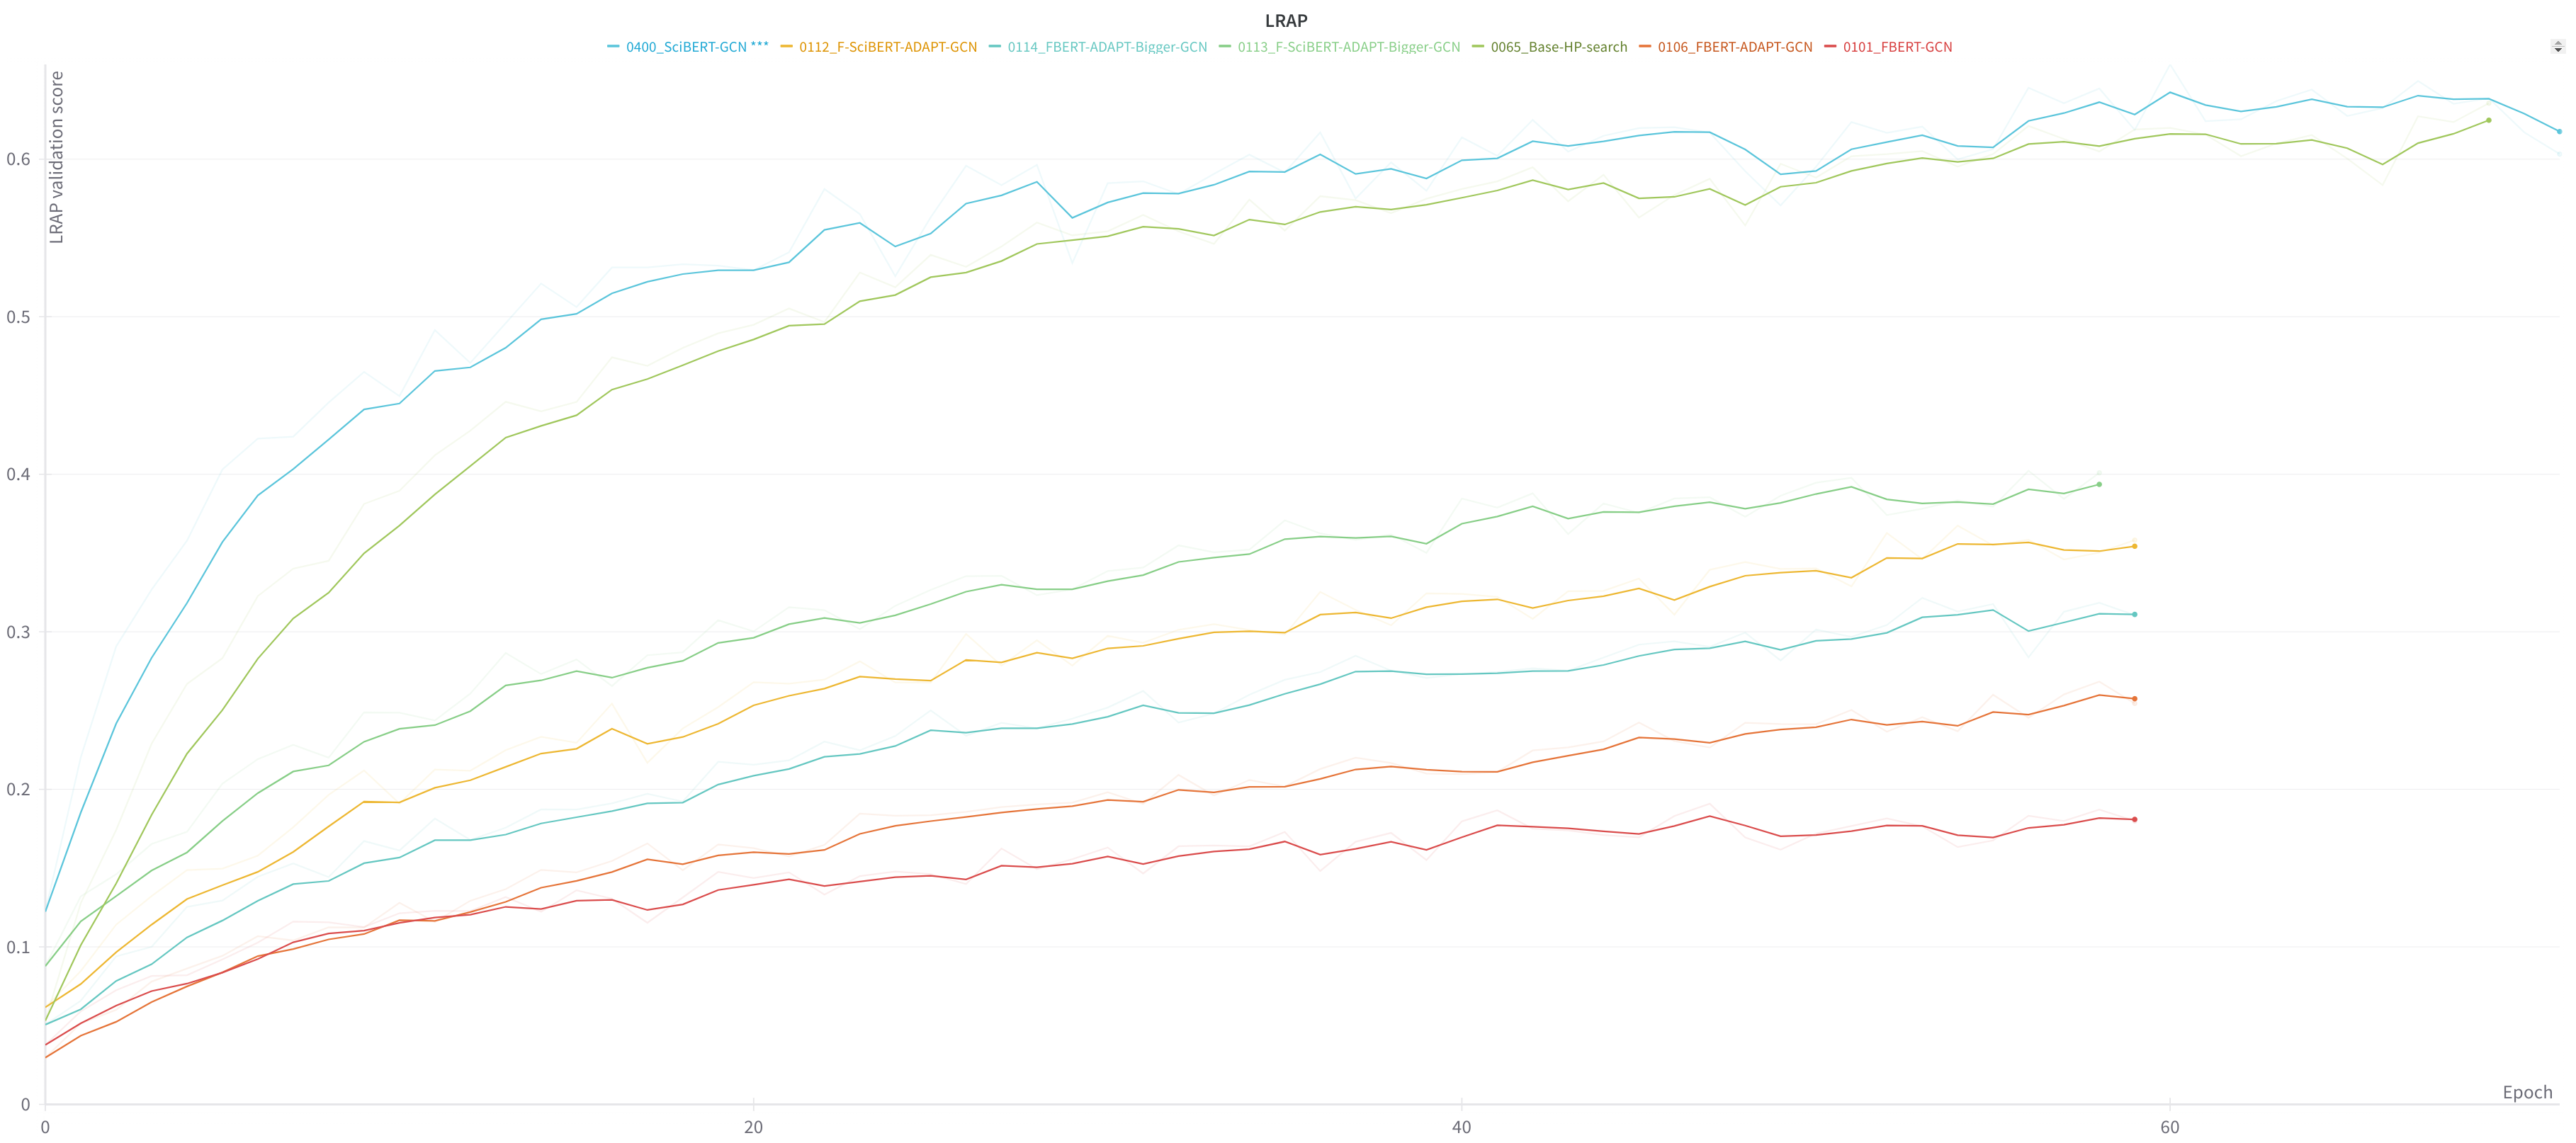
\includegraphics[width=1.\textwidth]{figures/preliminary_study.png}
    \caption{Training curves for the preliminary study.}
    \label{fig:preliminary_study_curves}
\end{figure*}

